入力層:ニューロン数は960(一次元画像データの値の数).

中間層:ニューロンの数を100から1100まで変更して,シミュレーションした.Fig.\ref{anti_left}の横軸は中間層ニューロンの数,
縦軸は左のモーターの予測出力と教師データ出力の平均二乗誤差.
Fig.\ref{anti_right}の横軸は中間層ニューロンの数,縦軸は右のモーターの予測出力と教師データ出力の平均二乗誤差.
中間層のニューロンの数の増加に従って,回帰誤差の増減に規則性はみられない.
経験によって,中間層のニューロンの数を1000にした.

出力層:左右のモーターの制御パワーを計算するので,出力層ニューロンの数が2にする.

活性化関数:relu関数.

最適化アルゴリズム:Adamでバッチ学習である.

Adamのパラメーター: $\alpha$=0.01,$\eta$=0.3,$\beta$1=0.9,$\beta$2=0.9,$\epsilon$=$1\times e^{-8}$.$w$=0.

Fig.\ref{LeftOutput}とFig.\ref{rightOutput}は学習終わったニューラルネットワークの回帰結果部分的グラフです.
横軸はデータの番号(1番目から600番目の教師データをグラフした),
縦軸は左のモーターの出力(Fig.\ref{LeftOutput})と右のモーターの出力(Fig.\ref{rightOutput})です.
%オレンジ色の線が教師データの出力で,青色線が教師データと同じの入力(1次元画像データ)でニューラルネットワークの予測出力です.
ニューラルネットワークの予測出力が教師データの出力に完璧に回帰していないと見られるけど,
人間のラジコンで収集した教師データも完璧ではないと考えて,ある程度回帰できれば,実際の走行実験の振舞いで評価するにした.

\vspace{-2mm}
\begin{figure}[h]
        \centering
        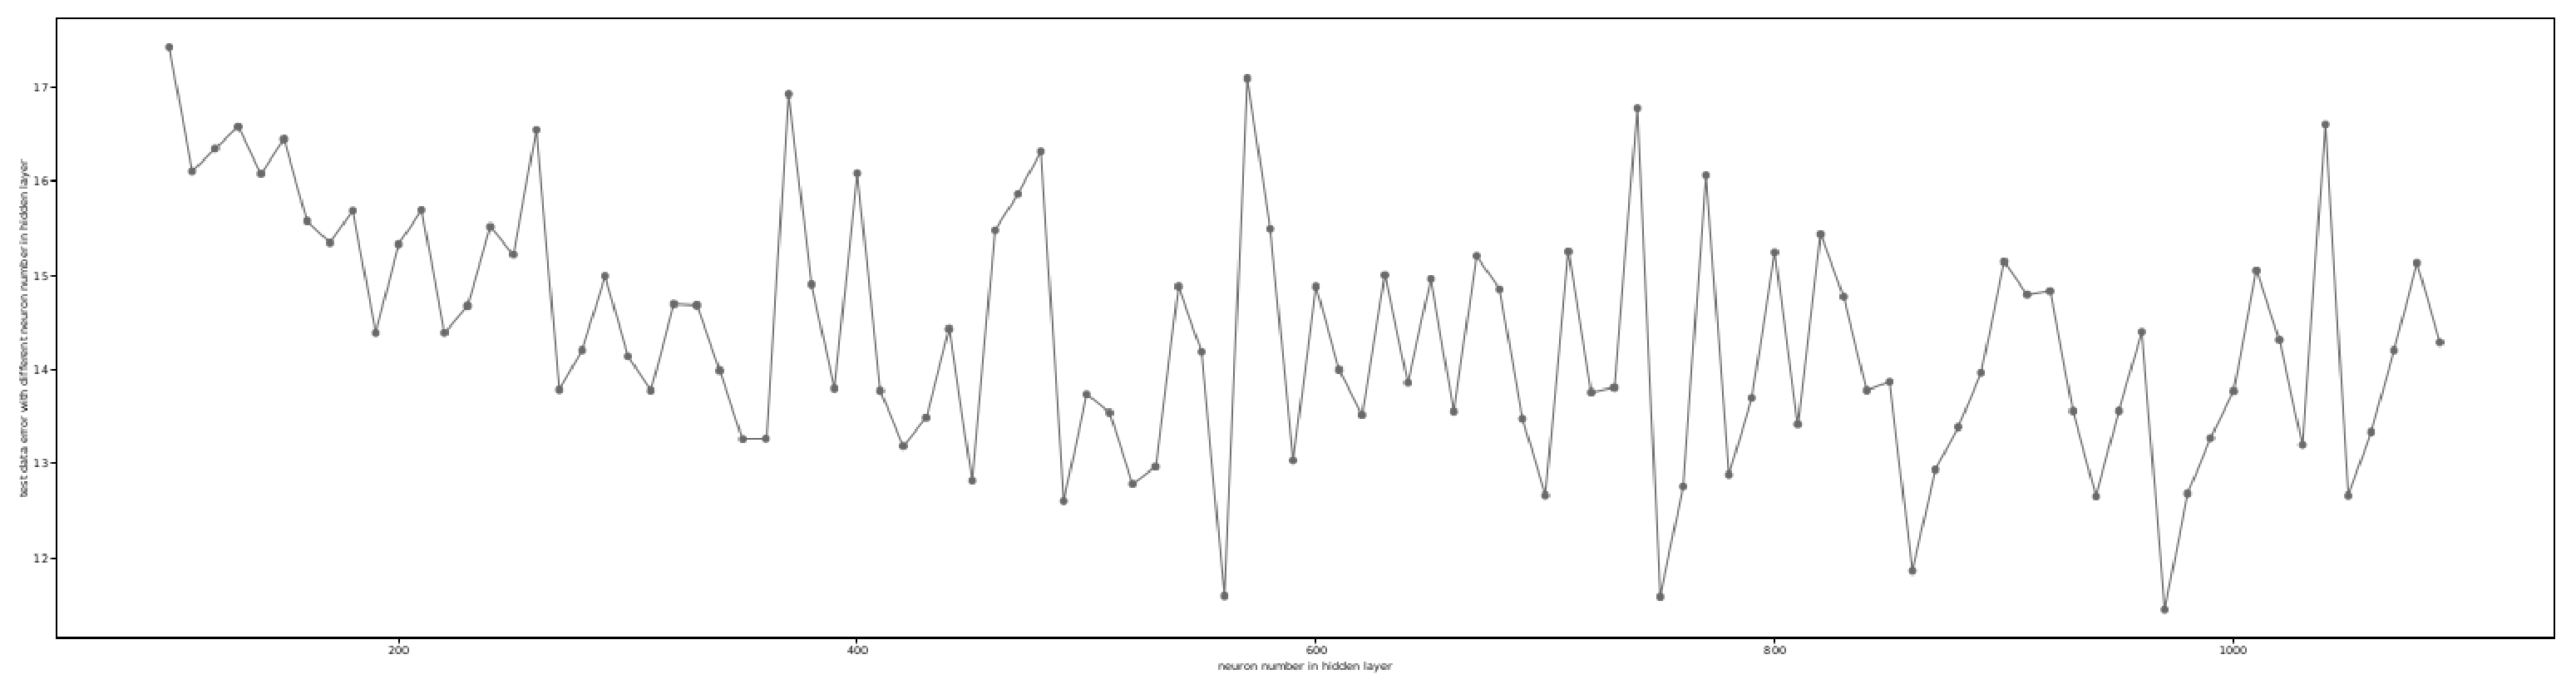
\includegraphics[width=1.0\linewidth]{anti_left.eps}
        \caption{中間層ニューロンの数と左のモーターの出力誤差}
        \label{anti_left}
\end{figure}
\vspace{-5mm}
\begin{figure}[h]
        \centering
        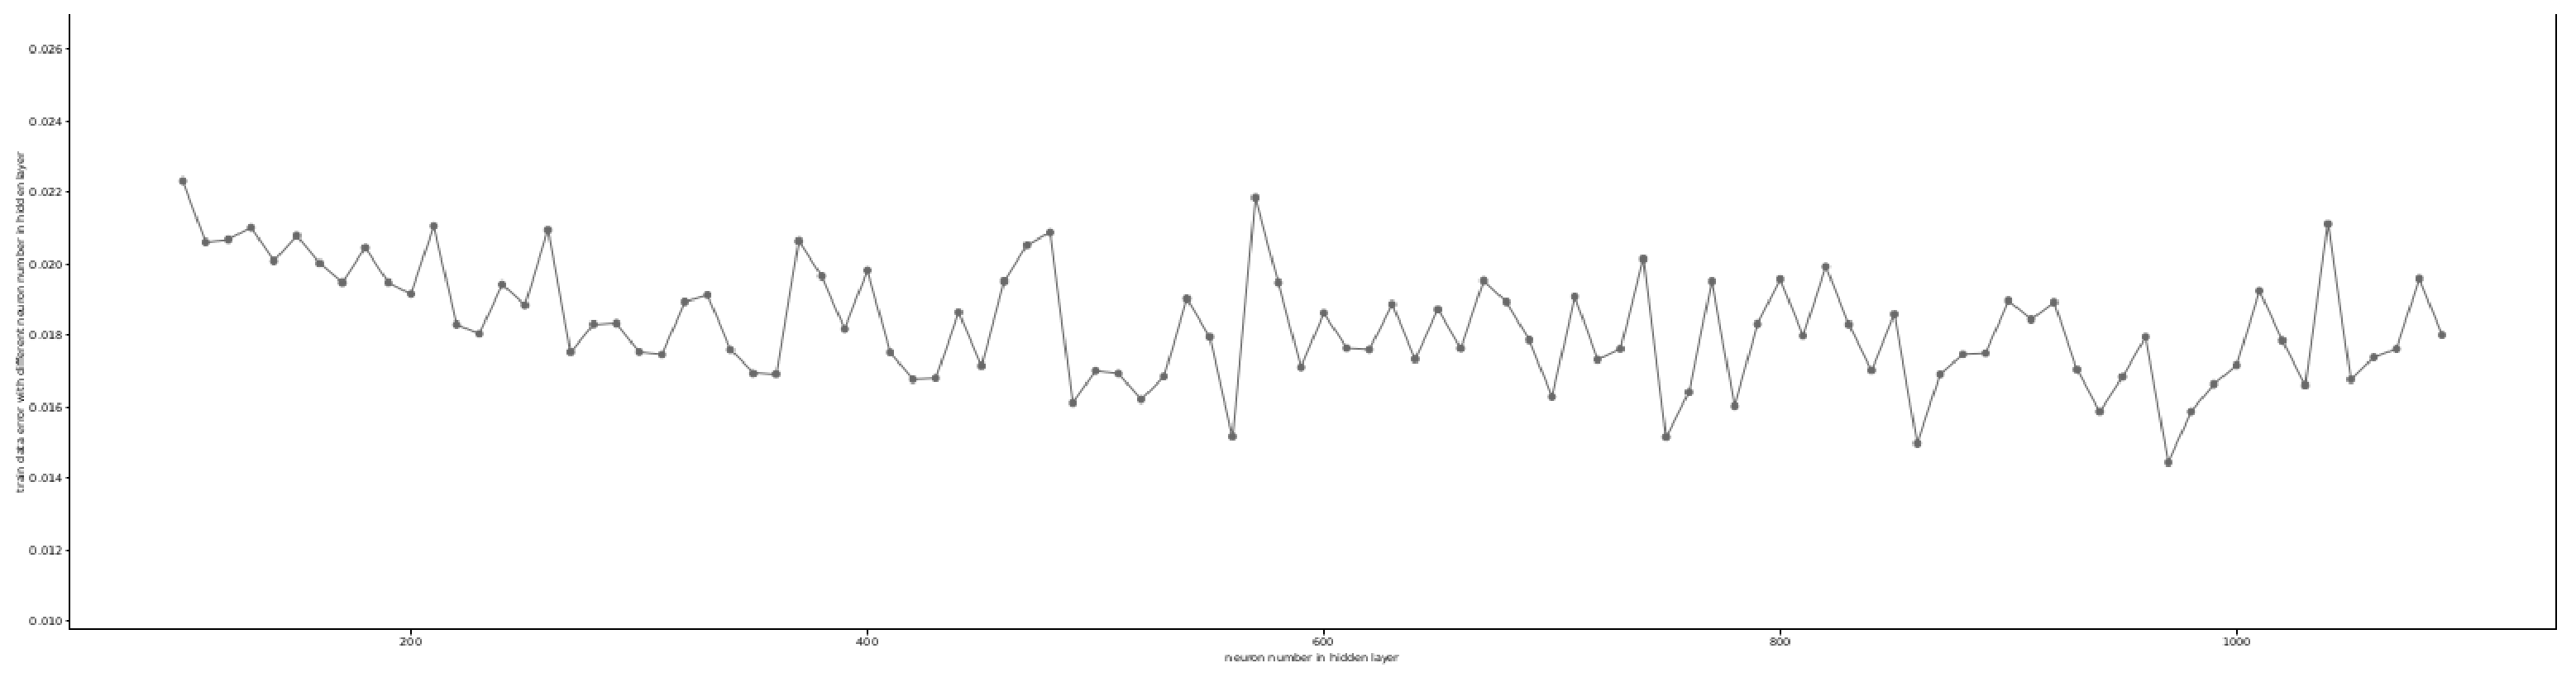
\includegraphics[width=1.0\linewidth]{anti_right.eps}
        \caption{中間層ニューロンの数と右のモーターの出力誤差}
        \label{anti_right}
\end{figure}

\vspace{-7mm}
\begin{figure}[!ht]
    \centering
    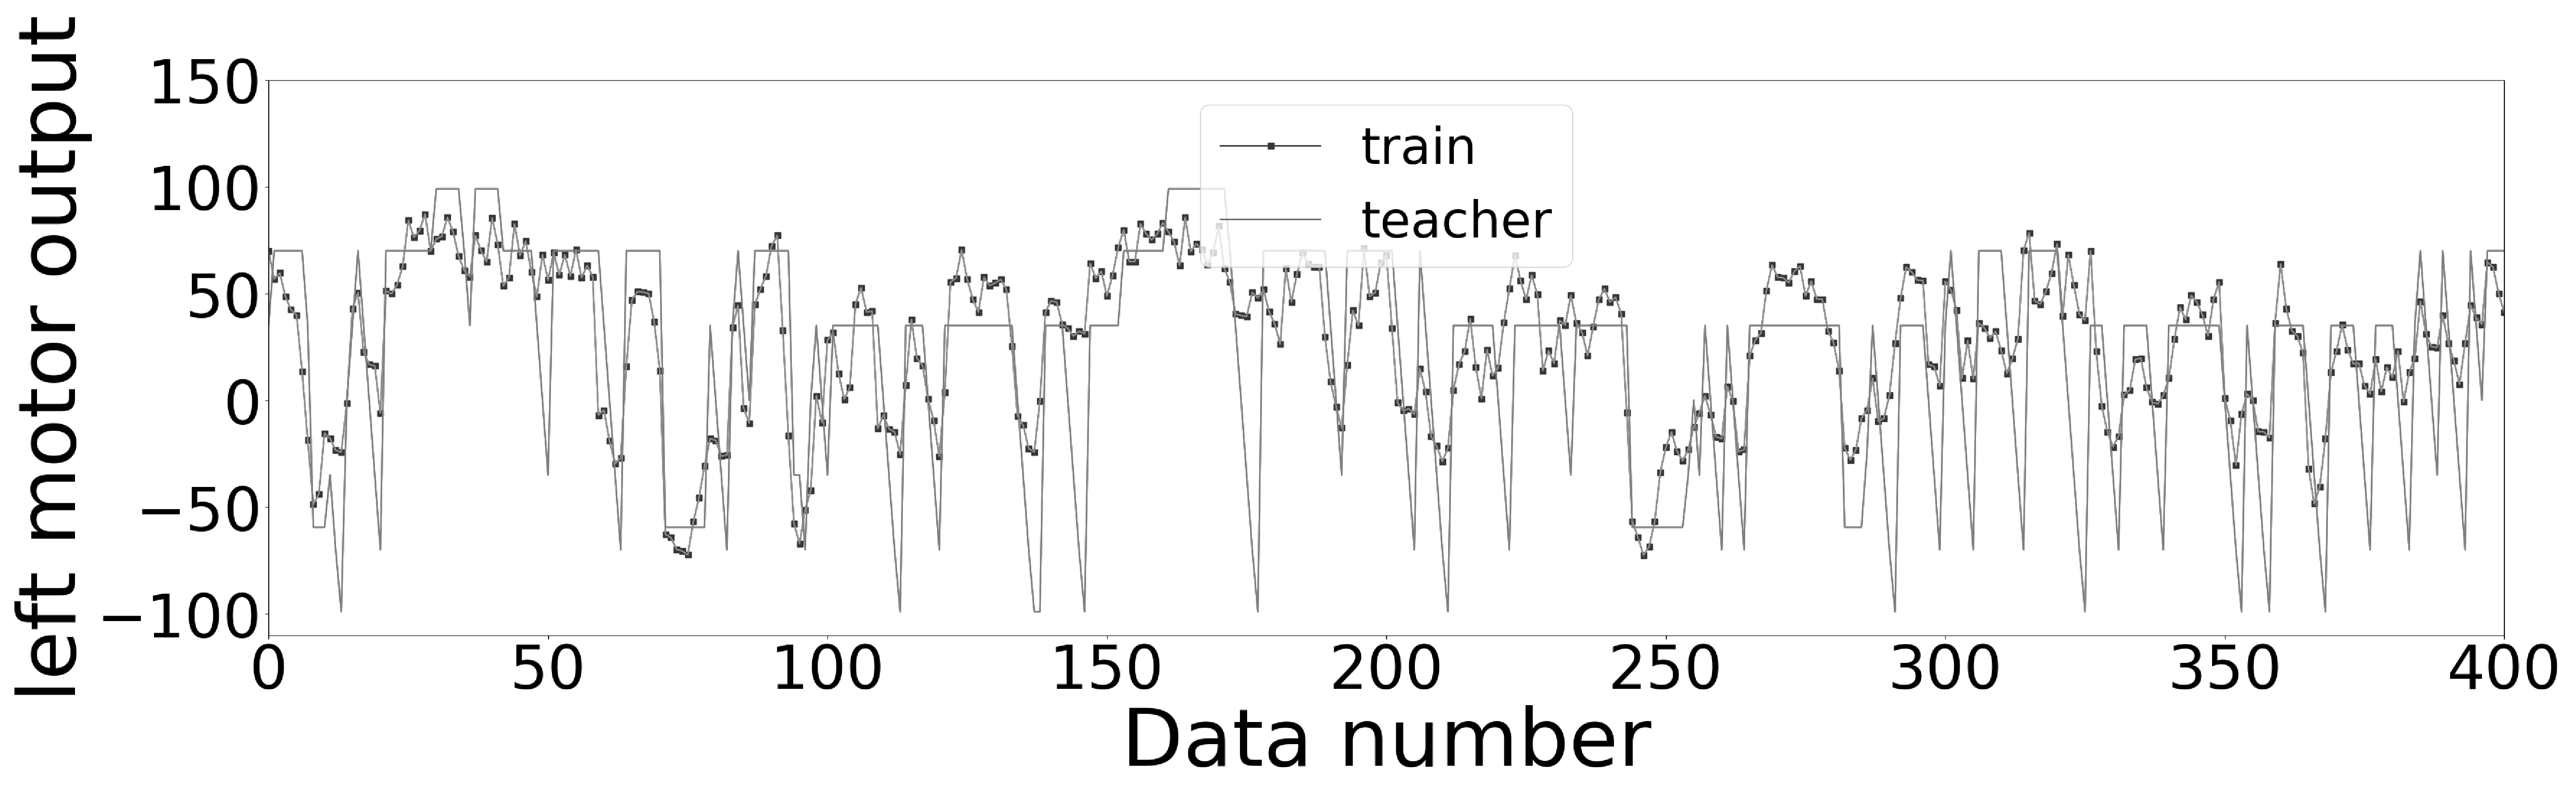
\includegraphics[width=1.0\linewidth]{LeftOutput.eps}
    \caption{NNで左のモーターの出力の回帰結果(局部)}
    \label{LeftOutput}
\end{figure}

\vspace{-7mm}
\begin{figure}[!ht]
    \centering
    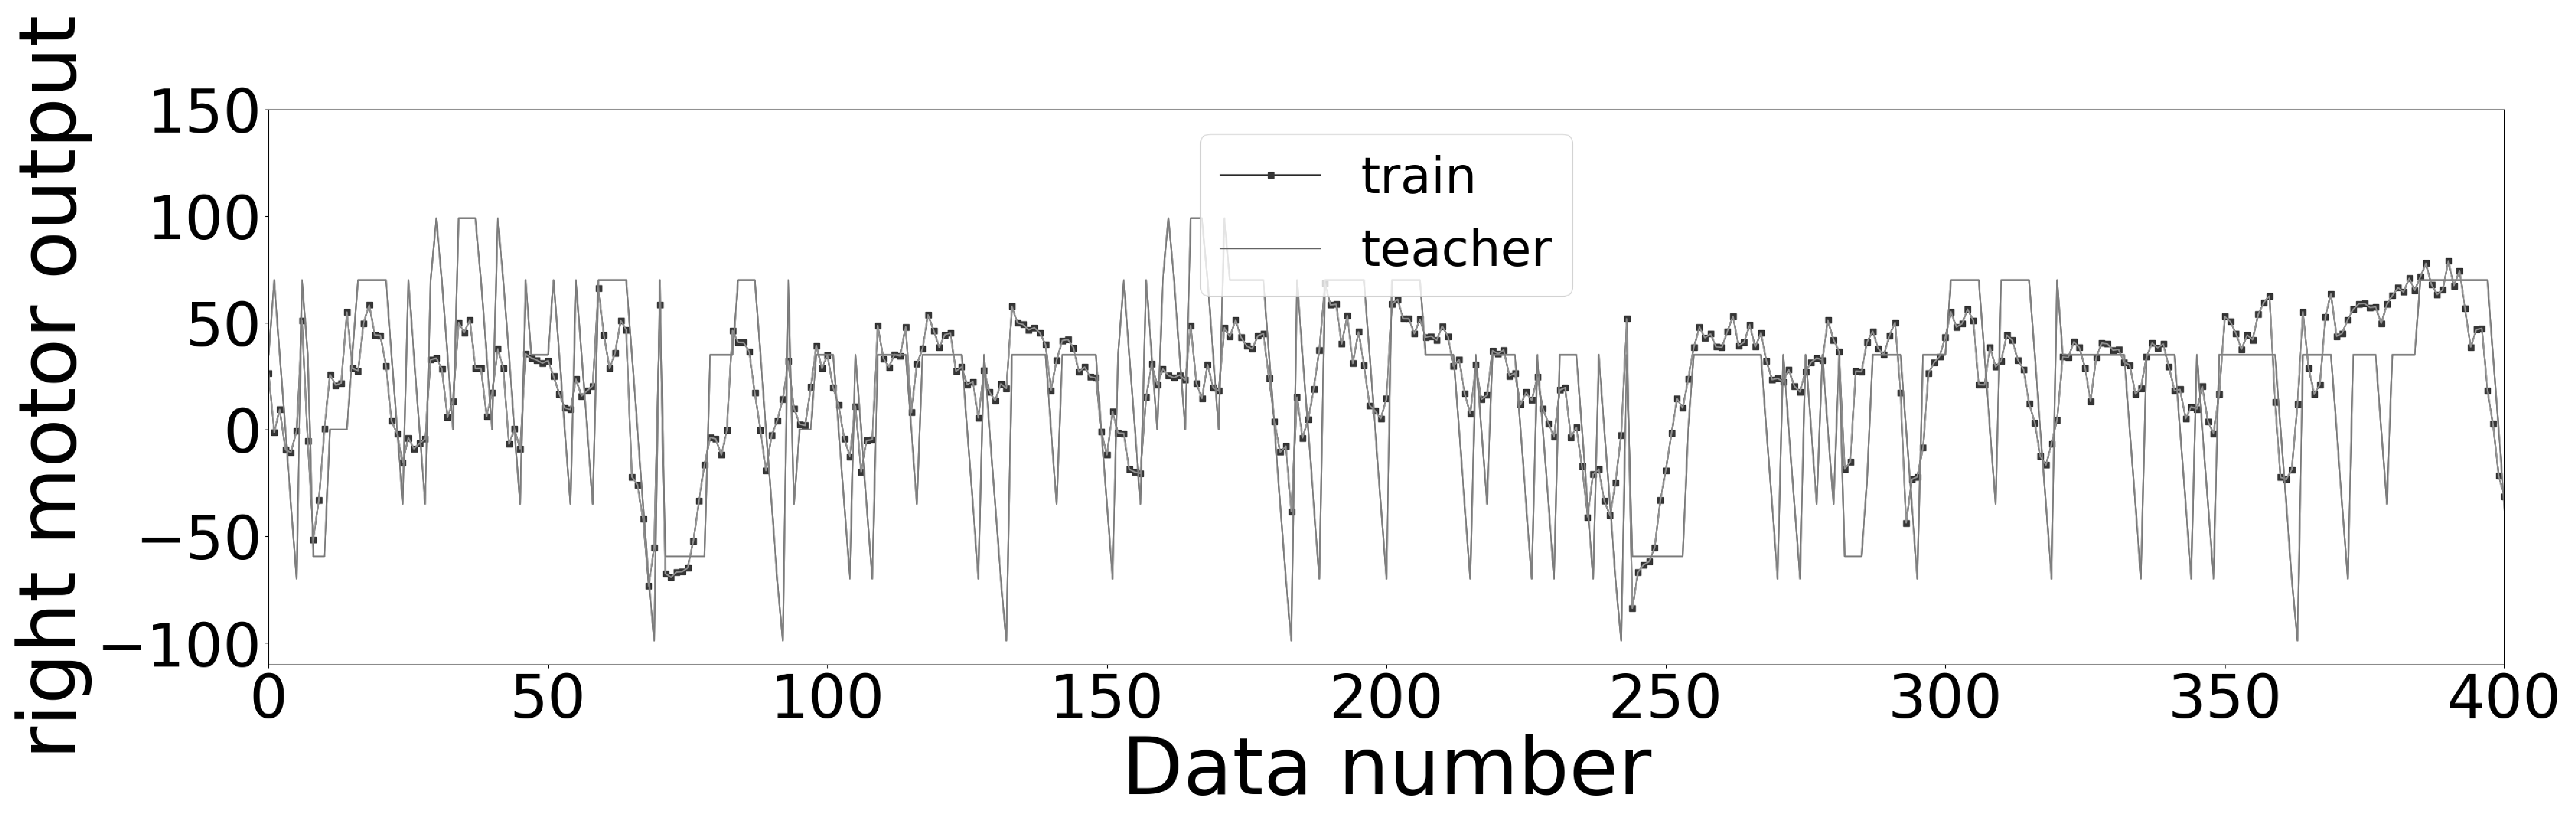
\includegraphics[width=1.0\linewidth]{rightOutput.eps}
    \caption{NNで右のモーターの出力の回帰結果(局部)}
    \label{rightOutput}
\end{figure}
